\chapter{Metodologia}
Nesse seção apresentamos a Metodologia.

Usamos o modelo da rede convolucional-LSTM proposto por \cite{FullResolution2017Toderici} cuja arquitetura foi apresentada em \ref{fig:toderici3} com algumas modificações. 

O método de reconstrução de uma imagem $x$ será aditivo e a rede aprende a reconstruir a informação residual. Além disso, em um dado estágio ou iteração $t$, o autocodificador recebe a diferença entre o resíduo da iteração anterior $r_{t-1}$ e a sua previsão $r'_{t-1}$. Essas duas características estão resumidas na próxima Equação, em um estágio:

\begin{equation}
\label{eq:model_1it}
\begin{aligned}
r_{0} &=x\\
x'_0  &=0 \\
b_{t} &= B(E_{t}(r_{t-1})) \\
r'_{t-1} &= D_{t}(b_{t}) \\
r_{t} &= r_{t-1}- r'_{t-1} \\
x'_t &= r'_{t-1} + x'_{t-1}  
\end{aligned}
\end{equation}




Usamos as camadas Conv2DLSTM descritas pela Equação \ref{eq:conlstm} para capturar as dependências espaciais dos resíduos. A figura \ref{fig:convlstm} detalha essa camada com $k$ mapas de recursos. 

\begin{figure}[ht]
	\centering
	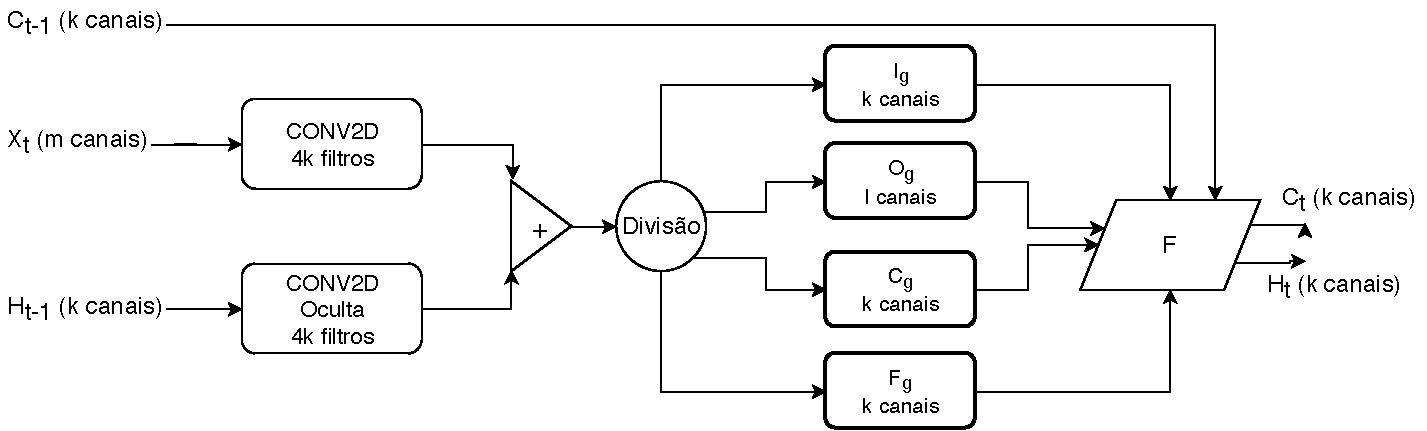
\includegraphics[width=0.90\textwidth]{figuras/convlstm.pdf}
	\caption[Conv2DLSTM]{Camada convolucional recorrente com $k$ filtros. Sendo $X_t$ o elemento atual da nossa sequencia com $m$ canais que está sendo processado, $H_{t-1}$ e $c_{t-1}$ representam a saída e estado de célula gerados por essa unidade na etapa anterior. As saídas de ambas as convoluções tem o mesmo número de canais,$4\times k$, para serem somadas ponto-a-ponto. Em seguida, o novo tensor é separado em 4 novos tensores de k canais. Eles representarão as portas de entrada, esquecimento, célula e saída. A função F irá operar as portas e em conjunto com $C_{t-1}$ para fornecer $C_t e H_t$ segundo as equações em \ref{eq:conlstm}.}
	\label{fig:convlstm}
\end{figure}

A Figura \ref{fig:rede_toderici} mostra a rede ``desenrolada'' no tempo. Para simplificar a representação omitimos as camadas profundidade para espaço.

\begin{figure}[htbp]
	\centering
	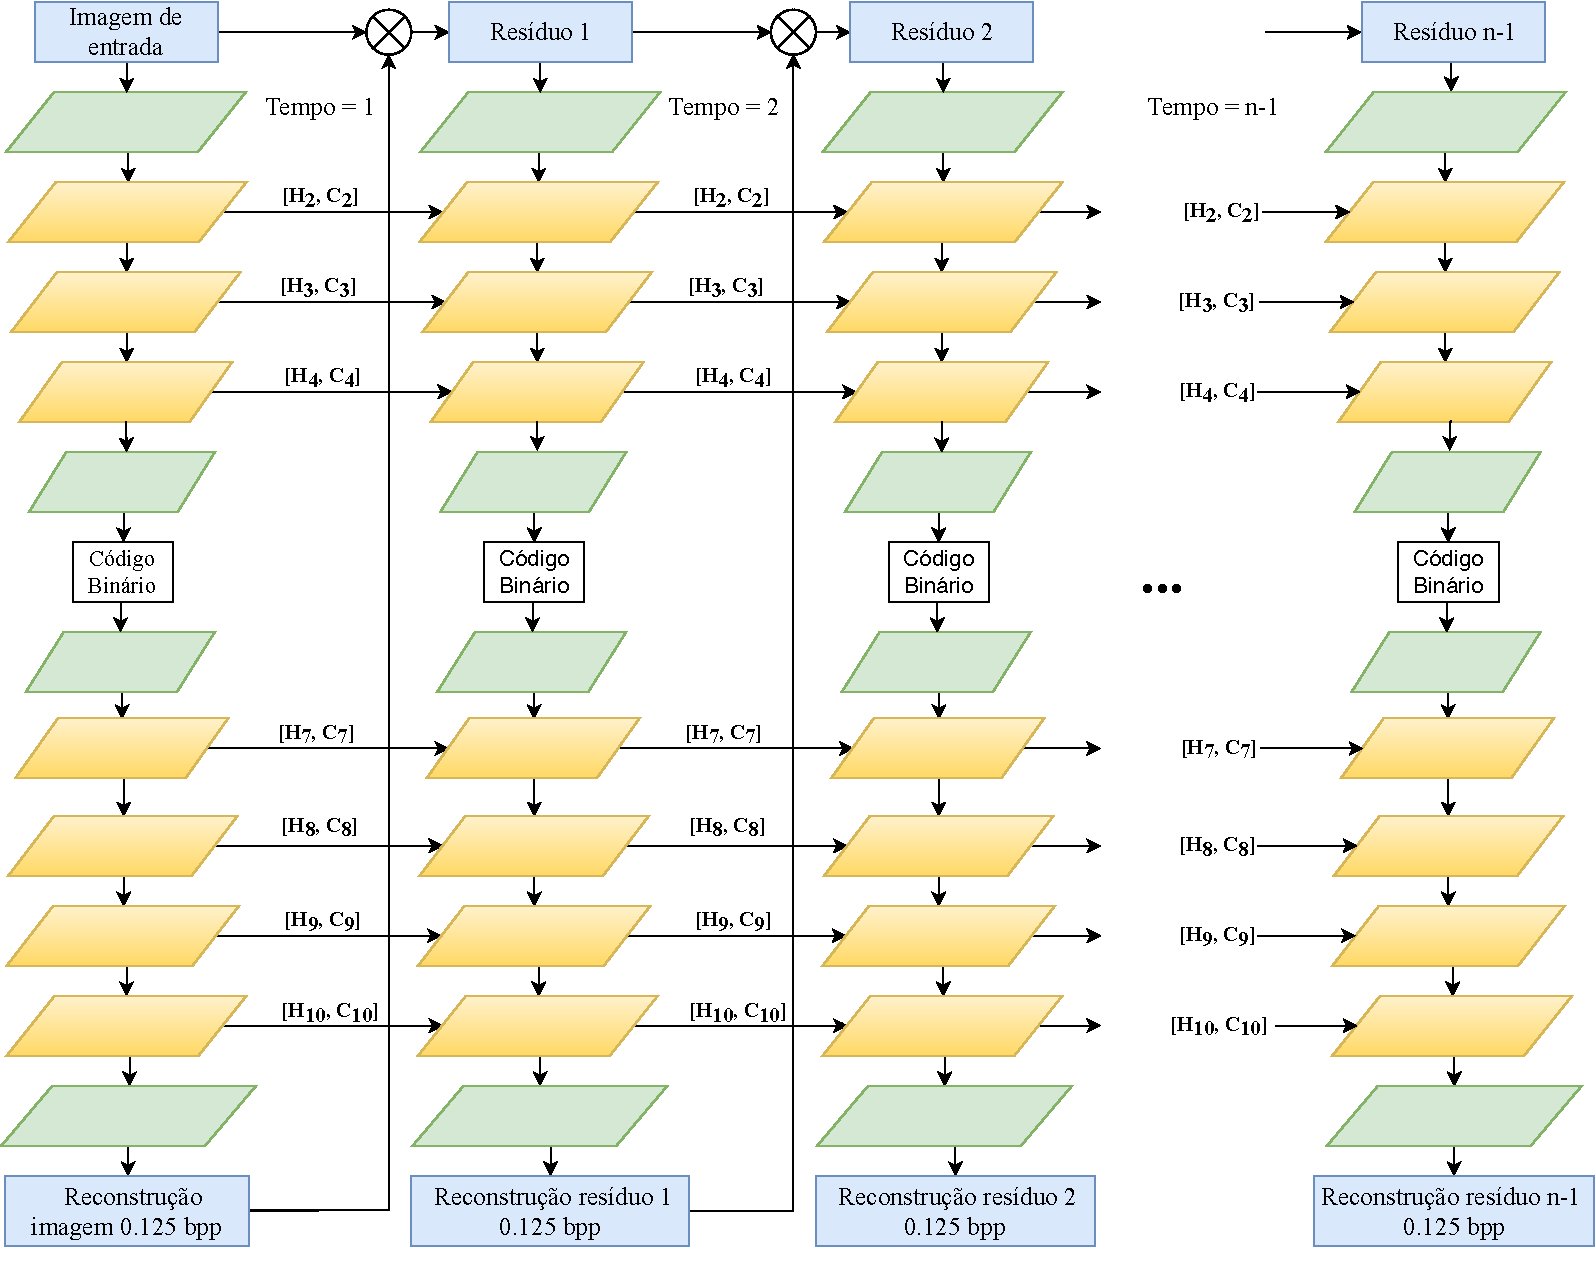
\includegraphics[width=0.90\textwidth]{figuras/redeTCC.pdf}
	\caption[Autocodificador desenrolado no tempo]{Representação do autocodificador no decorrer de $n$ estágios. Os losangos verdes e laranjas representam as camadas Conv2d e Conv2DLSTM, respectivamente.  Na primeira iteração os valores de $C_t e H_t$ para cada Conv2DLSTM são zeros e as setas horizontais evidenciam o $loop$ dessas camadas. Em cada interação o autocodificador recebe o resíduo da reconstrução anterior como entrada e tenta reconstrói-lo ao final da iteração usando 0,125 bits por pixel.}
	\label{fig:rede_toderici}
\end{figure}


Por construção, a arquitetura da rede determina que a saída do codificador fornece um conjunto de bits da forma $\frac{H}{16} \times \frac{W}{16} \times 32$ por iteração em que $H$ e $W$ são, respectivamente, a altura e largura da imagem de entrada. Isso nos fornece $\frac{H \times W}{8}$ bits e podemos calcular a taxa nominal por iteração $R_{it}$ em bits por pixel:

\begin{equation}
\label{eq:bpp}
R_{it} = \frac{\frac{H \times W}{8}}{H \times W} =  \frac{1}{8}\text{ bpp} 
\end{equation}

Então, obtemos a taxa nominal $R$ na iteração $k>0$ como $R =\frac{k}{8} $.  Dessa forma podemos controlar a quantidade de bits por pixel que enviamos ao decodificador com o passo de $1/8$. 


Aplicando a Equação \ref{eq:compressao} obtemos a  taxa compressão nominal $C$ na iteração $k$: 

\begin{equation}
\label{eq:tc}
C = \frac{24 \times H \times W}{k \times \frac{H \times W}{8}} =  \frac{192}{k} 
\end{equation}


Os detalhes do autocodificador podem ser consultados na Tabela \ref{table:aerc} considerada entradas formadas por blocos de imagens $32 \times 32 \times 3$. O tamanho do minilote está omitido dessa representação, contudo,  ele ocupa mais uma dimensão de valor fixo durante todas as operações realizadas pela rede.

\begin{table}[htbp]
	\caption{Parâmetros das operações no autocodificador.}
	\begin{tabular}{|c|c|c|c|c|c|c|}
		\hline
		\rowcolor[HTML]{EFEFEF} 
		\textbf{Camada} & \textbf{\begin{tabular}[c]{@{}c@{}}Formato de\\  saída\end{tabular}} & \textbf{\begin{tabular}[c]{@{}c@{}}Núcleo \\ Convolucioal\\ Normal/Oculto\end{tabular}} & \textbf{Passo} & \textbf{Preenchimento} & \textbf{\begin{tabular}[c]{@{}c@{}}Função de\\ Ativação\end{tabular}} & \textbf{\begin{tabular}[c]{@{}c@{}}Número de\\ Parâmetros\end{tabular}} \\ \hline
		Conv2D          & 16x16x64                                                             & 3x3/-                                                                                   & 2              & ``Mesmo''                   & Identididade                                                          & 1728                                                                    \\ \hline
		Conv2DLSTM      & 8x8x256                                                              & 3x3/1x1                                                                                 & 2              & ``Mesmo''                   & Sigmoid                                                               & 851968                                                                  \\ \hline
		Conv2DLSTM      & 4x4x512                                                              & 3x3/1x1                                                                                 & 2              & ``Mesmo''                   & Sigmoid                                                               & 5767168                                                                 \\ \hline
		Conv2DLSTM      & 2x2x512                                                              & 3x3/1x1                                                                                 & 2              & ``Mesmo''                   & Sigmoid                                                               & 10485760                                                                \\ \hline
		Conv2D          & 2x2x32                                                               & 1x1/-                                                                                   & 1              & ``Válida''                  & Tanh                                                                  & 16384                                                                   \\ \hline
		Binarizador     & 2x2x32                                                               & -                                                                                       &                &                        &                                                                       &                                                                         \\ \hline
		Conv2D          & 2x2x512                                                              & 1x1/-                                                                                   & 1              & ``Mesmo''                   & Identididade                                                          & 16384                                                                   \\ \hline
		Conv2DLSTM      & 2x2x512                                                              & 3x3/1x1                                                                                 & 1              & ``Mesmo''                   & Sigmoid                                                               & 10485760                                                                \\ \hline
		P.E             & 4x4x128                                                              & -                                                                                       &                &                        &                                                                       &                                                                         \\ \hline
		Conv2DLSTM      & 4x4x512                                                              & 3x3/1x1                                                                                 & 1              & ``Mesmo''                   & Sigmoid                                                               & 3407872                                                                 \\ \hline
		P.E             & 8x8x128                                                              & -                                                                                       &                &                        &                                                                       &                                                                         \\ \hline
		Conv2DLSTM      & 8x8x256                                                              & 3x3/1x1                                                                                 & 2              & ``Mesmo''                   & Sigmoid                                                               & 1441792                                                                 \\ \hline
		P.E             & 16x16x64                                                             & -                                                                                       &                &                        &                                                                       &                                                                         \\ \hline
		Conv2DLSTM      & 16x16x128                                                            & 3x3/1x1                                                                                 & 2              & ``Mesmo''                   & Sigmoid                                                               & 360448                                                                  \\ \hline
		P.E             & 32x32x32                                                             & -                                                                                       &                &                        &                                                                       &                                                                         \\ \hline
		Conv2D          & 32x32x3                                                              & 1x1/-                                                                                   & 1              & ``Mesmo''                   & Tanh                                                                  & 96                                                                      \\ \hline
		\multicolumn{6}{|c|}{Total de parâmetros}                                                                                                                                                                                                                                                          & 32835360                                                                \\ \hline
	\end{tabular}\quad
	\label{table:aerc}
\end{table}


O processo de binarização adotado foi o descrito na seção \ref{subsec:bin} e proposto em \cite{Variable2016Toderici}.


%\section{Taxas de compressão}




%A Figura \ref{fig:modelo} mostra a arquitetura de uma única iteração do nosso modelo.  Nela temos 4 camadas no encoder: 3 convolucionais e 1 RNN-Conv; 1 camada de binarização do tipo convolucional; e 6 camadas no enconder: 2 convolucionais e 4 unidades RNN-Conv.  As camadas convolucionais são utilizadas especialmente para extrair os recursos das imagens essenciais para garantir a reconstrução de imagens com a menor perda possível. Já as camadas recorrentes do tipo LSTM são empregadas para capturar as dependências entre os patches de entrada e os resíduos gerados nas iterações.   

%\begin{figure}[h]
%	\centering
%	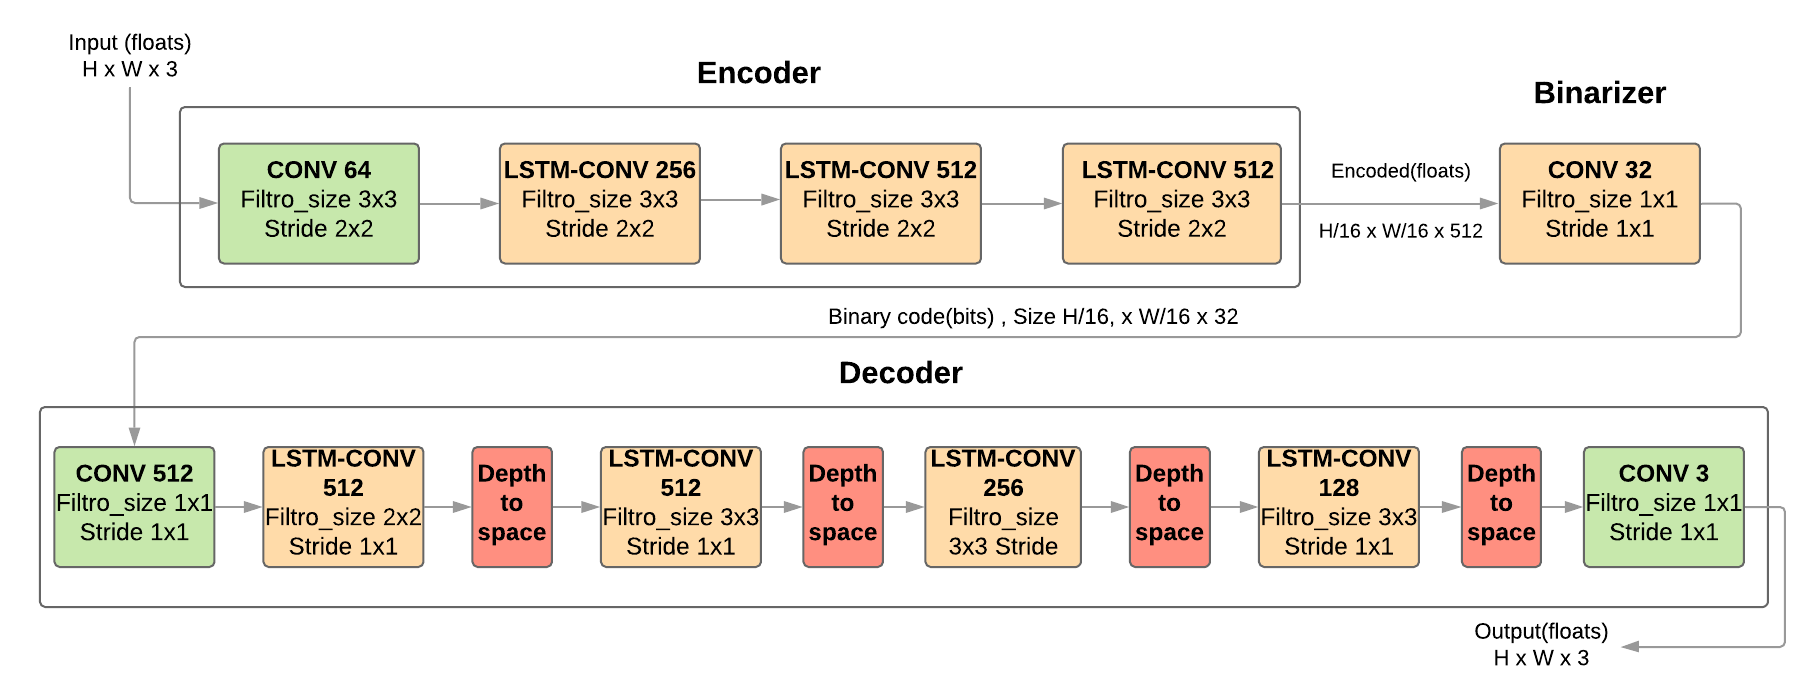
\includegraphics[width=0.90\textwidth]{figuras/arquitetura_rede.png}
%	\caption{Representação de uma iteração do autoencoder \cite{Variable2016Toderici}.}
%	\label{fig:modelo}
%\end{figure}




%Nas unidades RNN-Conv ilustradas na figura \ref{fig:modelo} o tamanho do filtro e o stride refere-se a primeira convolução, a segunda convolução sempre terá filtros de dimensão 1x1 com stride 1x1; e o número de filtros refere-se ao número de canais da LSTM e 1/4 do número de canais das camadas convolucionais dessa unidade.



\section{Formato do fluxo de bits}

A arquitetura é otimizada para reconstruir blocos de $32 \times 32 \times 3$ uma vez que foi treinada com imagens dessa dimensão. Portanto, dividimos nossa imagem para gerar blocos $32 \times 32$. Vamos nos referir a cada um dos blocos por $b_p$ em que $p \in \{0,...,n-1\}$ em que $n$ foi o número de blocos obtidos. 
Considerando um lote de tamanho $l$ no qual vamos fazer $k$ iterações na rede.  Na primeira iteração da rede o codificador irá tomar os primeiros $l$ blocos na ordem direita para esquerda e de cima para baixo e passar pela rede do codificador para gerar o código binário parcial de formato $l \times 2 \times 2 \times 32$ conforme a tabela \ref{table:aerc}. Em seguida, decodificamos esse lote e computamos o resíduo. Esse resíduo é codificado para gerar um novo código binário $l \times 2 \times 2 \times 32$ que é concatenado com o anterior para formar $2 \times l \times 2 \times 2 \times 32$. 
Esse processo se repete até concluirmos as $k$ iterações na rede, e ao final da codificação de um lote o nosso código binário é da forma $k \times l \times 2 \times 2 \times 32$. 
O número de vezes que temos repetir o processo descrito acima para codificar a imagem inteira é de $\frac{n}{l}$. Portanto, o código binário final é da forma $\frac{n}{l} \times k \times l \times 2 \times 2 \times 32$. Obviamente, o número de bits desse código independe do tamanho de lote escolhido. 


\section {Base de Dados}

Idealmente, desejamos obter uma base de dados de treinamento a fim de tornar o modelo capaz de comprimir satisfatoriamente (desempenho semelhante ao JPEG) imagens naturais com diferentes características de tamanho, componentes de frequência, entropia etc. Essa é uma das principais escolhas para treinar qualquer algoritmo de redes neurais.  
Intuitivamente, formaremos a base de dados de treinamento com imagens que não passaram por nenhum processo de compressão com perdas. Dessa forma, acreditamos ela seja mais representativa por preservar todas as componentes de frequência das imagens naturais. A partir dela são construídas novas bases de dados com blocos de características distintas de entropia. A hipótese é, baseado em \cite{Variable2016Toderici,FullResolution2017Toderici}, que a performance do autocodificador está relacionado com essa característica. O processo de construção das bases de dados a seguir foram obtidas seguindo o relatório técnico em \cite{DeliverableJuly}.

Primeiro, uma base de dados principal foi obtida usando todas as imagens dos seguintes conjuntos de dados:

\begin{enumerate}
	\item Conjunto de dados CLIC \cite{bib:clic} (\textit{Challenge on Learned Image Compression}) - Imagens de alta qualidade.
	\subitem \textit{Professional} - validação: 41 imagens
	\subitem \textit{Professional} - treinamento: 585 imagens;
	\subitem \textit{Mobile} - validação: 61 imagens;
	\subitem \textit{Mobile} - treinamento: 1048 imagens.
	\item Conjunto de dados DIV2K \cite{bib:div2k} (\textit{DIVerse 2K resolution high.
		quality image}) - Imagens de alta resolução
	\subitem Treinamento: 800 imagens;
	\subitem Validação: 100 imagens.
	\item Conjunto de dados Ultra-Eye \cite{bib:ultraeye} (\textit{Ultra-Eye: UHD and HD images eye tracking datase}) - Alta qualidade e alta resolução.
	\subitem HD: 38 imagens;
	\subitem UHD: 40 imagens.
\end{enumerate}

As imagens foram separadas em blocos de $32 \times 32 \times 3$ os quais foram salvos usando compressão sem perdas no padrão PNG. Esse procedimento gerou 6.231.440 blocos.
Apresentamos na Figura \ref{fig:histdatabase} um histograma do tamanho desses blocos. Essa medida será usado como uma estimativa da entropia do bloco.

\begin{figure}[htbp]
	\centering
	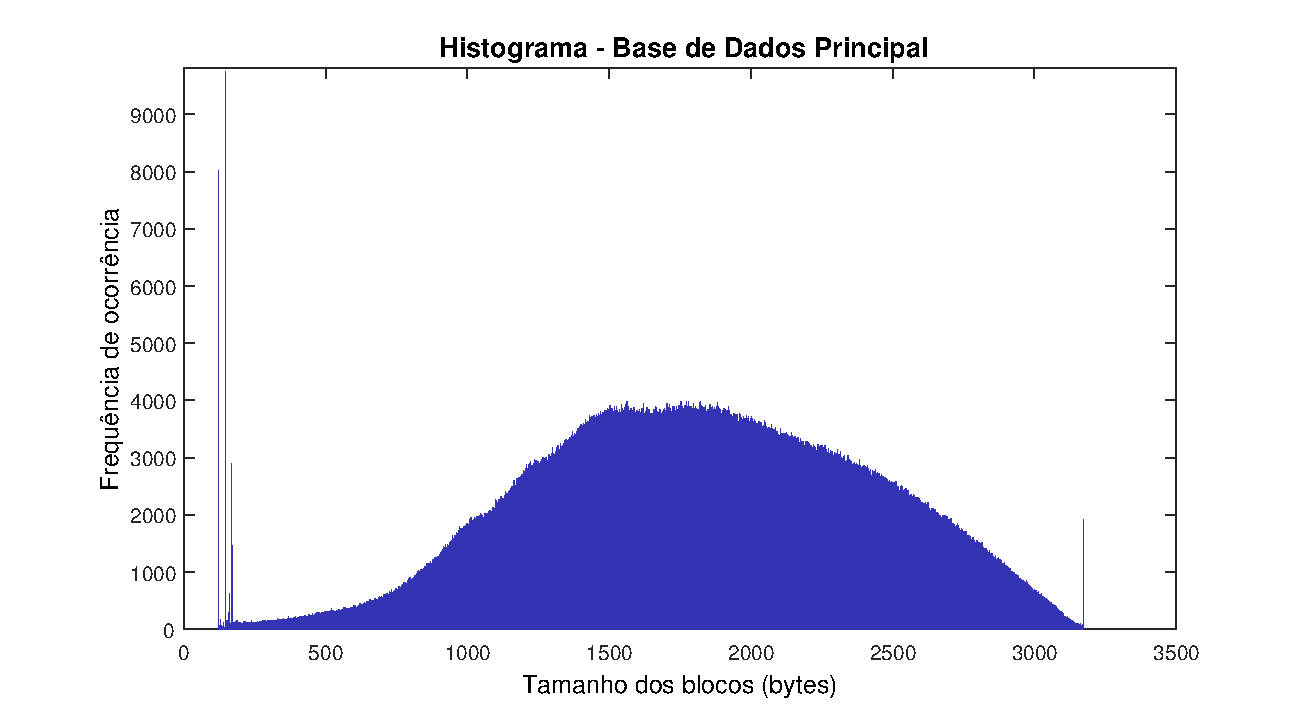
\includegraphics[width=0.80\textwidth]{figuras/hist.eps}
	\caption{Histograma de todo o banco de dados}
	\label{fig:histdatabase}
\end{figure}

O bloco que apresentou maior entropia foi definido como uma referência de entropia igual a 100\%. 
A partir dessa referência, e tendo em mente que a entropia das imagens de treinamento impactaria na performance do modelo, separamos os blocos em 5 base de dados observando os seguintes critérios:

\begin {enumerate}
\label{list:bds}
\item Banco de dados 0 (BD0). Todos os blocos cuja entropia seja menor que 20\% do valor da entropia de referência. Total: 1.248.978 blocos. 
\item Banco de dados 1 (DB1). Todos os blocos no intervalo de 40\% e 60\% de entropia de referência. Total: 1.251.421 blocos.
\item Banco de Dados 2 (DB2). Todos os blocos correspondentes a pelo menos 80\% da entropia de referência. Total: 1.248.725 blocos.
\item Banco de Dados 3 (DB3). Sorteio de 20\% dos blocos que compõem toda a base de dados. Total: 1.247.033 blocos
\item Banco de Dados 4 (DB4). Sorteio de 20\% dos blocos cuja entropia varia de 50\% a 100\%. Total: 1.246.698 blocos
\item Banco de Dados 5 (DB5). Todos os blocos cuja entropia varia de 50\% a 100\% em relação a nossa referência. Total: 2.287.520 blocos
\end{enumerate}


Por construção, não há sobreposição entre os bancos de dados 0, 1 e 2. No entanto, existem sobreposições de informações entre os bancos de dados 3 e 4. Os histogramas dessas bases, exceto a 5, estão ilustrados nas Figuras \ref{fig:database0}, \ref{fig:database1}, \ref{fig:database2}, \ref{fig:database3} e \ref{fig:database4}.



\begin{figure}
\centering
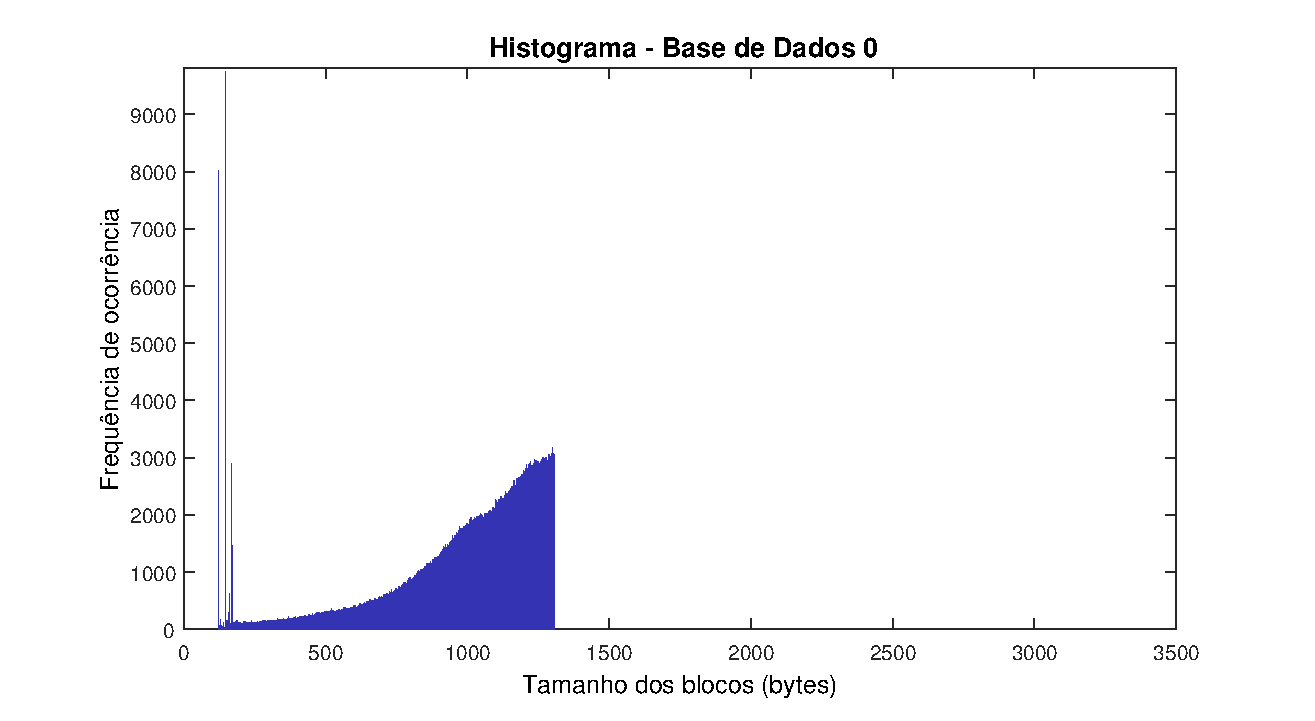
\includegraphics[width=0.8\textwidth]{figuras/hist0.eps}
\caption{Histograma da baixa entropia DB0.}
\label{fig:database0}
\end{figure}

\begin{figure}
\centering
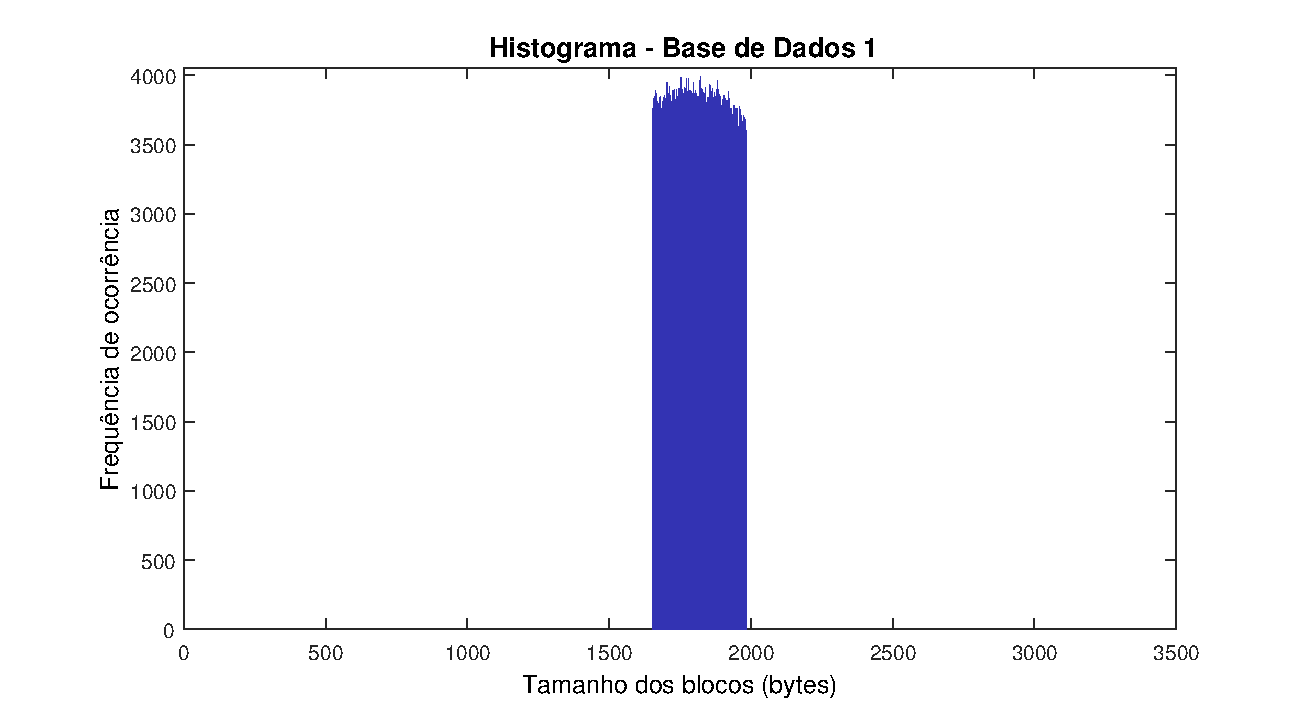
\includegraphics[width=0.80\textwidth]{figuras/hist1.eps}
\caption{Histograma do DB1 de entropia média.}
\label{fig:database1}
\end{figure}

\begin{figure}
\centering
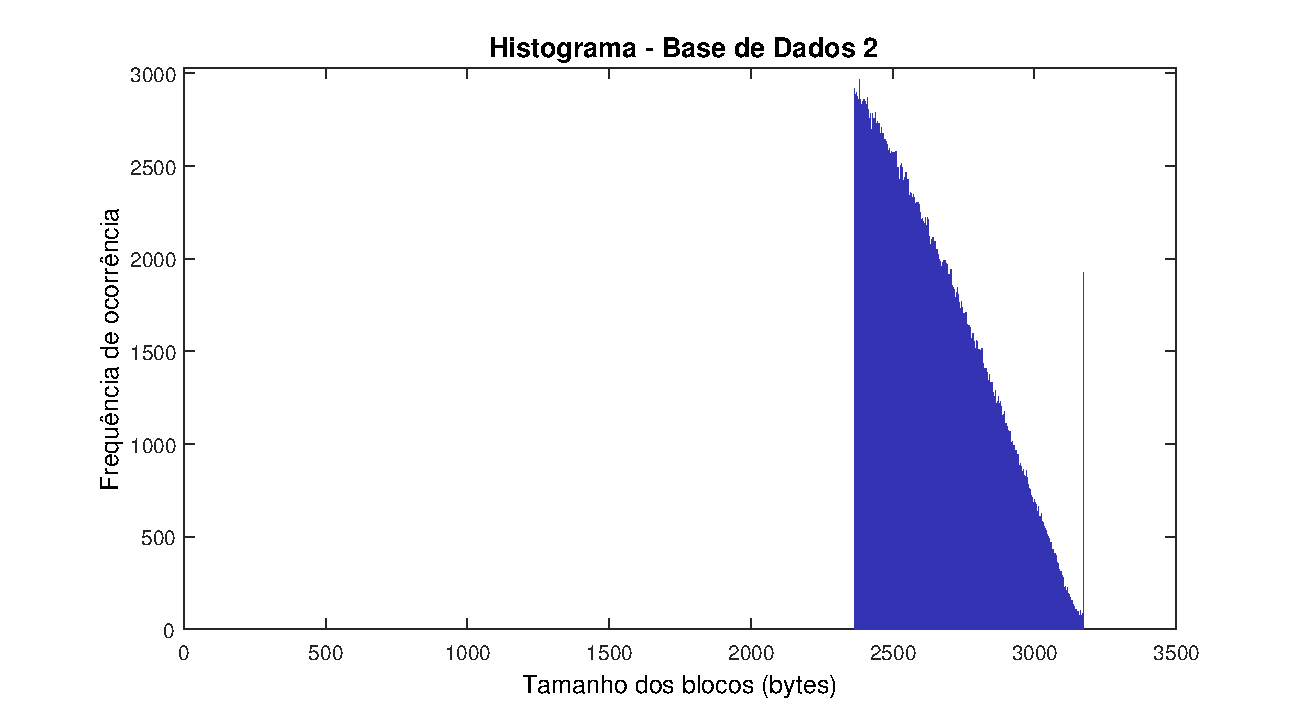
\includegraphics[width=0.8\textwidth]{figuras/hist2.eps}
\caption{Histograma do DB2 de alta entropia.}
\label{fig:database2}
\end{figure}

\begin{figure}
\centering
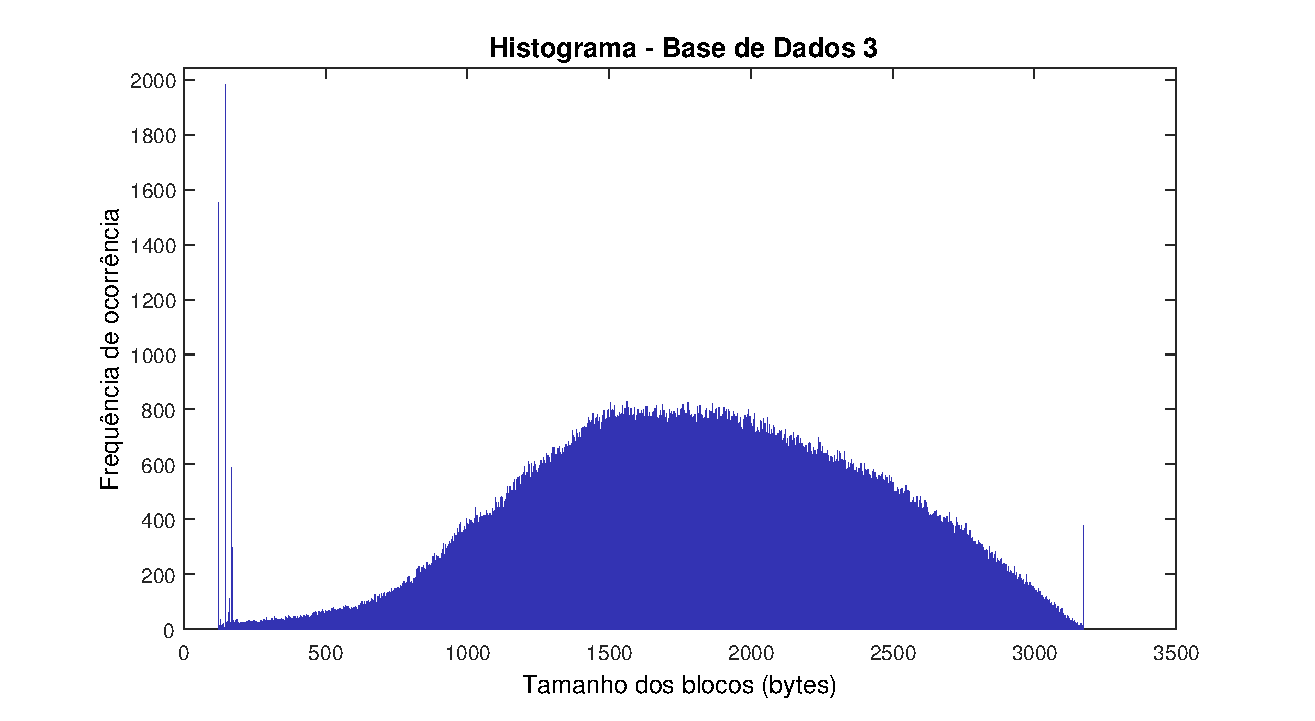
\includegraphics[width=0.80\textwidth]{figuras/hist3.eps}
\caption{Histograma da entropia mista DB3.}
\label{fig:database3}
\end{figure}

\begin{figure}
\centering
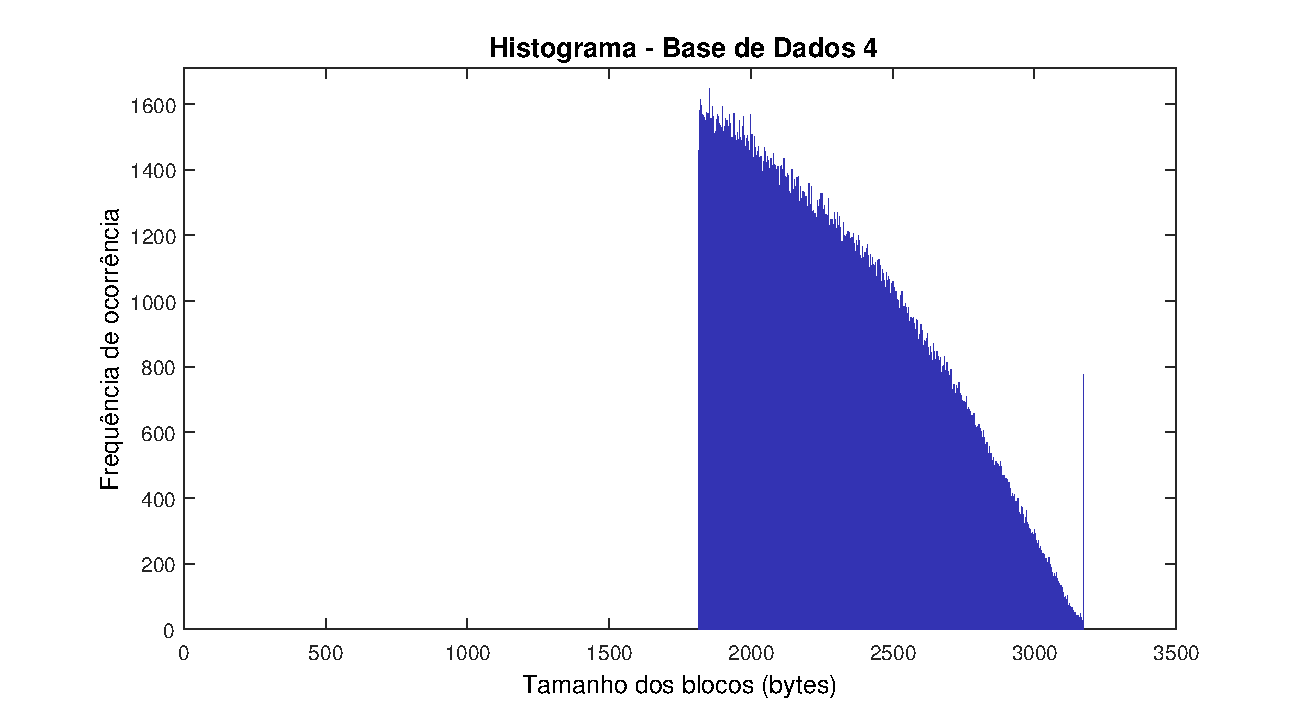
\includegraphics[width=0.8\textwidth]{figuras/hist4.eps}
\caption{Histograma da entropia alta DB4.}
\label{fig:database4}
\end{figure}		

A base de dados da Kodak \cite{kodak} formada por 24 imagens naturais foi empregada nos testes do autocodificador.  

\section {Função de Custo}

A função de custo é outra escolha importante nos treinamento de RNA. No problema de compressão de imagens a escolha dessa função tem o agravante de não haver consenso entre os pesquisadores de uma métrica ideal para avaliar a qualidade entre uma imagem original e a sua versão reconstruída como relatado em \cite{Priming2017Johnston,End2016Balle}.  
%Na hipótese de haver tal função, poderíamos definir uma função de erro em relação a métrica ideal como função de custo e minimizar o seu valor ao longo do aprendizado do modelo. 
Algumas funções conhecidas apresentam relações da medida de distorção entre uma imagem e sua reconstrução, tais como $MSE$, $MAE$, e versões diferenciáveis de $1-SSIM$ e $1-MS-SSIM$. Em nossos testes, dedicamos atenção especial na escolha da função de custo conveniente para o problema de compressão de imagens. No primeiro momento,
avaliamos a performance do modelo com  distorção das reconstruções.

Vamos definir algumas variações e combinações dessas funções e comparar os resultados em treinamentos curtos.
A função de custo $L$ é calculada em cada estágio e ao final das iterações computamos a sua média para finalmente aplicar os algoritmos de retropropagação e atualização dos pesos, isto é:

\begin{equation}
l = \frac{1}{k} \sum_{t=0}^k L(r_t,r'_t) 
\end{equation}


Até aqui, não estamos tendo controle sobre a entropia do código binário gerado. Se pudermos otimizar a rede para gerar a sequência de bits com baixa entropia teremos ganhos relevantes ao aplicador um codificador de entropia.

Portanto, em um segundo momento adicionamos uma função de regularização $R$ para otimizar implicitamente a taxa do código binário, inspirado no trabalho \cite{zhao1901cae}. 
Para calcula-lo fazemos uma cópia do código binário fornecido pela função de binarização em um dada iteração $t$, $B(E_t(r_{t-1}))$, para a variável $Z$. Nessa variável, substituímos os bits -1 por 0 e aplicamos a norma $L_1$ sobre $Z$. Ademais, empregamos a função MSE como um medida de distorção para obter a nova função de perdas $L$:   

\begin{equation}
\label{eq:rdo}
L = MSE(r,r') + \lambda(t) \times \sum_{t=1}^{n} Z 
\end{equation}


onde $n$ é o número de bits do código binário por nível. Em nossa rede esse número é igual a 128 por bloco $32x32$. A ideia é que ao penalizarmos a ocorrência do bit 1 estamos, essencialmente, reduzindo a entropia de ordem 0 do código binário. Esperamos que isso reflita na redução da taxa ao aplicarmos um codificador de entropia.   

O fator e $\lambda(t) >0$ é uma regularização que controla a proporção de $R$ sobre a função de custo e que depende da iteração. Em nossos testes, verificamos é interessante que $\lambda$ seja uma função decrescente da iteração $t$. Para um mini-lote de blocos de treinamento, à medida que as iterações prosseguem o resíduo reconstruído se torna cada vez menor e consequentemente a distorção medida pela MSE decaí. Todavia, tal comportamento não é esperado para a função $R$ e então controlamos o seu impacto em $L$ usando um valor de regularização menor. Dessa forma, tentamos balancear o impacto da distorção e taxa.  
Nessa abordagem, aplicamos uma codificação sem perdas dada pelo GZIP para aproveitar a estatística de distribuição do bits que esperamos ser de baixa entropia. Portanto, na reconstrução de uma imagem existe a taxa nominal $r_n$ e fixa por iteração, caracterizando um método de taxa $r_r$ constante (do inglês \textit{Constant bitrate} (CBR))), e há a taxa real fornecida pelo GZIP. O ganho percentual de taxa em virtude da codificação de entropia é descrito pela Equação a seguir:
\begin{equation}
\label{eq:gain_ce}
G = 100 \times \frac{r_n-r_r}{r_n}
\end{equation}




\section{Alocação dinâmica de bits}\label{sec:adb}
Uma desvantagem do modelo é que ele reserva um número fixo de bits para reconstruir qualquer bloco de imagem, independentemente da complexidade do seu conteúdo. Tal problema foi levantando em \cite{Priming2017Johnston} e descrito na revisão desse trabalho. Para tentar contornar essa desvantagem, propomos uma heurística simples e semelhante a \cite{Priming2017Johnston}.

O método de alocação dinâmica de bits é uma etapa realizada após o treinamento da rede. Nele, ao final de cada iteração e para cada lote de blocos $32 \times 32$ que são passados pela rede do codificador e decodificador calculamos a sua média de PSNR e desse conjunto também obtemos a menor PSNR. Se essa média for maior ou igual a um alvo de qualidade ($P_{a}$) e a menor PSNR for maior ou igual a $P_{ct}$\% do valor desse alvo então interrompemos a reconstrução nesse ponto e passamos a codificar o próximo lote. Se chegarmos no número máximo iterações ($k_{max}$) codificaremos o próximo lote.
Como veremos, essa prática gera imagens com artefatos de blocos que comprometam a qualidade perceptual ainda que a PSNR indique melhora. Por isso, adicionamos mais uma restrição: independentemente de $P_{a}$ haverá um número mínimo e máximo de iterações que os blocos estão sujeitos. O fluxograma na Figura \ref{fig:flux_vr} resume o método de alocação dinâmica de bits. 


\begin{figure}
\centering
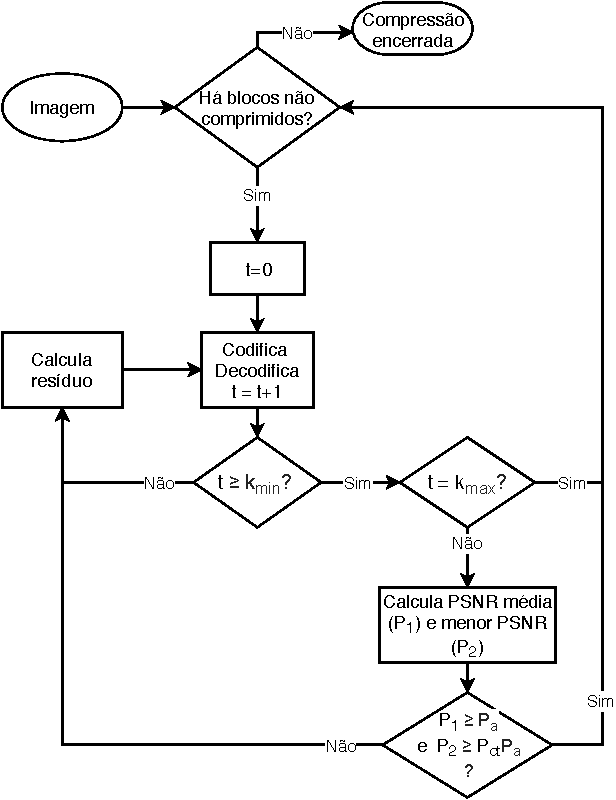
\includegraphics[width=0.7\textwidth]{figuras/fluxograma.pdf}
\caption{Alocação dinâmica de bits.}
\label{fig:flux_vr}
\end{figure}		


\section{Implementação}
O autocodificador foi implementado usando a biblioteca PyTorch da empresa Facebook.  Ele tem a vantagem de ter suporte a redes neurais construídas de forma dinâmica. Isso a torna a programação e depuração mais fácil e intuitiva em relação a biblioteca TensorFlow da Google. 
Nas demais tarefas como cálculo de métricas de qualidade e obtenção de curvas utilizamos, principalmente, a linguagem Python e Matlab na minoria das vezes.  
